\documentclass[compress,10pt,aspectratio=169]{beamer}
%\setbeamertemplate{background canvas}[bottom=white,top=structure.fg!25]
%\usetheme{Hannover}
\setbeamertemplate{headline}{}
\setbeamertemplate{footline}{June 27, 2020 - SDRA}
\setbeamersize{text margin left=0cm}
\usepackage{appendixnumberbeamer}
\usepackage{hyperref,listings,picinpar,mathtools} % ,enumitem}
\usepackage{color}
\settowidth{\leftmargini}{\usebeamertemplate{itemize item}}
\addtolength{\leftmargini}{\labelsep}

\definecolor{grey}{rgb}{0.95,0.95,0.95}
\definecolor{red}{rgb}{1.0,0.0,0.0}
\definecolor{green}{rgb}{0.0,0.6,0.0}
\definecolor{blue}{rgb}{0.0,0.0,1.0}
\lstloadlanguages{bash,Java,C,C++,csh,make,sh}%%[Visual]Basic,xml}
\lstset{frame=none,basicstyle=\footnotesize,breaklines,tabsize=2,captionpos=b,prebreak={\hbox{$\rightarrow$}},postbreak={\hbox{$\hookrightarrow$}},showstringspaces=false,backgroundcolor=\color{grey}\bfseries,keywordstyle=\color{blue},commentstyle=\color{green}\textit,stringstyle=\color{red}\ttfamily,abovecaptionskip=2pt,aboveskip=0pt,belowskip=0pt,belowcaptionskip=0pt}
%\lstset{moredelim=[is][\color{red}]{_+_}{_+_}}

\graphicspath{{../../figures/}}

\beamertemplatefootpagenumber
\beamertemplatenavigationsymbolsempty
\setbeamertemplate{footline}[page number]{}
\setbeamertemplate{page number in head/foot}{}

\usepackage{graphicx,verbatim,multicol,amsmath,bm}

\begin{document}

\title{Free, opensource Field Programmable Gate Array (FPGA) development frameworks for radiofrequency communication -- \\Digital communication using GNU Radio}
\author{N. Gallone, G. Goavec-Merou, J.-M Friedt\\ \ \\ 
FEMTO-ST/time \& frequency department \\ \ \\ jmfriedt@femto-st.fr \ \\ \ \\
slides and references at \url{https://github.com/oscimp/amaranth_twstft}}
\maketitle


\begin{frame}[fragile,noframenumbering]\frametitle{Architecture of an SDR transmitter}

\begin{itemize}
\item FPGA (Field Programmable Gate Array)-only SDR transmitter, no external analog component other
than a band-pass filter and antenna
\item Baseband information is frequency-transposed by mixing with a local oscillator (LO) to a 
radiofrequency band
\item IQ modulator requires generating a complex ($\exp(j\omega t$)) LO
\item LO is generated within the FPGA at a frequency limited to a fraction of the FPGA internal-clock frequency
\item square output on a FPGA General Purpose Intput Output (GPIO) pin allows for using harmonics if needed
\end{itemize}

\begin{center}
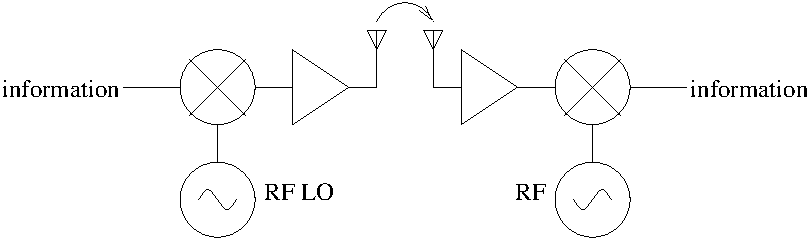
\includegraphics[width=0.6\linewidth]{chaine}
\end{center}
\end{frame}

\begin{frame}[fragile,noframenumbering]\frametitle{Outline}

How to generate a modulated radiofrequency signal on an FPGA configured as SDR transmitter?  

Amaranth (formerly nMignen) is selected for its 
\begin{itemize}
\item flexibility ({\bf Python-like} description of the hardware)
\item {\bf independence} from vendor-specific tools (Vivado framework, Mathworks HLS tools)
\item {\bf fast synthesis} for fast development cycle (program-simulate-test)
\item compatibility with a {\bf wide range} of lower-end FPGAs \footnote{\url{https://github.com/amaranth-lang/amaranth}}
\item practical demonstration on the Zynq7020 fitted on the Zedboard\footnote{\url{https://www.avnet.com/wps/portal/us/products/avnet-boards/avnet-board-families/zedboard/}}
\end{itemize}

\begin{center}
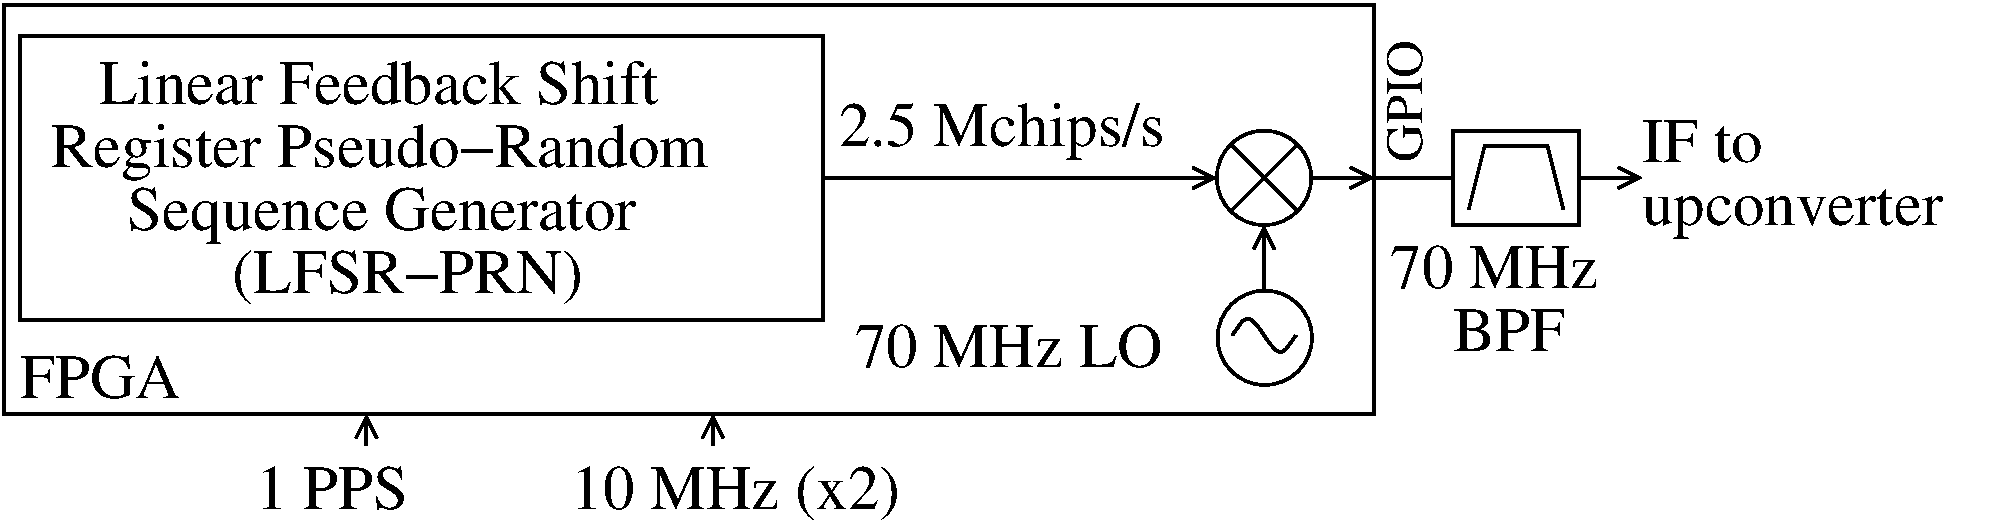
\includegraphics[width=0.6\linewidth]{../figures/setup.pdf}

\end{center}
\end{frame}

\begin{frame}[fragile,noframenumbering]\frametitle{Baseband signal structure}

\begin{itemize}
\item We select a pseudo-random sequence generated by a Linear Feedback Shift Register (LFSR) for assessing Bit Error 
Rate (BER) and used for ranging measurements
\item Accurate time of flight measured by correlating a local copy of the transmitter LFSR sequence
\item Modulation scheme: start with Binary Phase Shift Keying (BPSK), and later consider Quad-Phase Shift Keying (QPSK)
\end{itemize}

\begin{center}
\vfill
\input{lfsr.pspdftex}
\vfill
{\bf Getting started with FPGA basics and Amaranth programming}
\end{center}
\vfill
\end{frame}

\begin{frame}[fragile,noframenumbering]\frametitle{Baseband signal generation using Amaranth}

\begin{enumerate}
\item DONNER LES PRINCIPES D'AMARANTH, COMBINATOIRE v.s SYNCHRONE
\item SYNTAXE D'AMARANTH
\item COMMENT PROGRAMMER LE LFSR ET SIMULER LA SORTIE DANS GTKWAVE
\end{enumerate}
\end{frame}

\begin{frame}[fragile,noframenumbering]\frametitle{Baseband signal characterization (``random'' = no repeating pattern)}

Output sequence dumped as a binary file (here 10-bit long sequence)
\begin{lstlisting}[language=Python]
def write_prn_seq(file, bitlen, code, seed=1, mode=1, seqlen = 2500000):
  with open(file,"wb") as f:
    v = seed
    for i in range(seqlen):
      f.write((v%2).to_bytes(1,byteorder='big'))
      v = nextstate(v,code,bitlen)
    f.close()
\end{lstlisting}

\begin{minipage}[t]{\linewidth}
\begin{minipage}{.54\linewidth}
is read from Matlab or GNU/Octave with {\tt f=fopen('file.bin');c=fread(f,inf,'int8');}
\vspace{0.3cm}

Correlation: remove mean value {\tt c=c-mean(c);}
Signal Processing toolbox {\tt xcorr(code)}; or {\tt fcode=fft(code);iff(fcode.*conj(fcode));}
\begin{itemize}
\item autocorrelation and power spectrum density ...
\item ... using the simulation output or an FFT analyzer
\end{itemize}

\end{minipage}
\begin{minipage}{.45\linewidth}
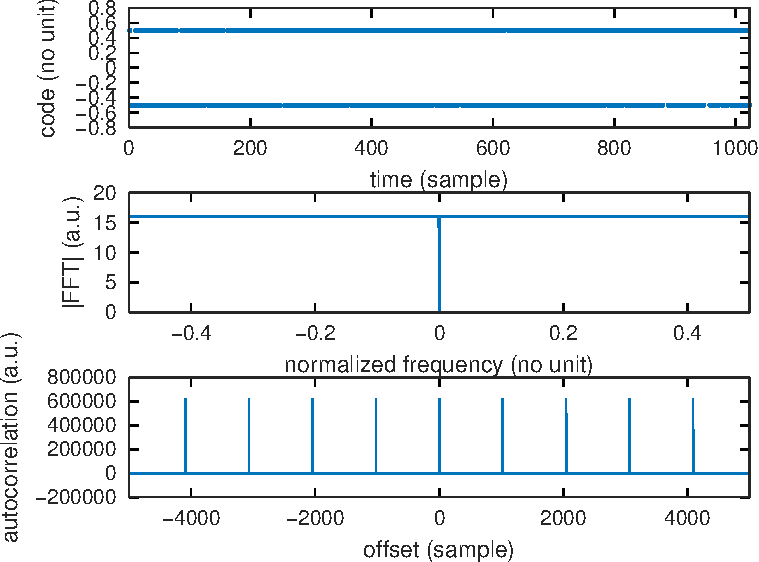
\includegraphics[width=1.05\linewidth]{10bitPRN.pdf}
\end{minipage}
\end{minipage}
\end{frame}

\begin{frame}[fragile,noframenumbering]\frametitle{Baseband signal characterization using GNU Radio}

\parbox{1.051\linewidth}{
Based on the convolution theorem $FFT(conv(x,y))=FFT(x)\cdot FFT(y)$ and
the close relation between convolution $conv(x,y)(\tau)=\int x(t)y(\tau-t)dt$ 
and correlation $xcorr(x,y)(\tau)=\int x(t)y(\tau+t)dt$ then
}
$$FFT(xcorr(x,y)(\tau))=FFT(t)\cdot FFT^*(y)$$

\vfill
\begin{minipage}[t]{1.1\linewidth}
\begin{minipage}{.49\linewidth}
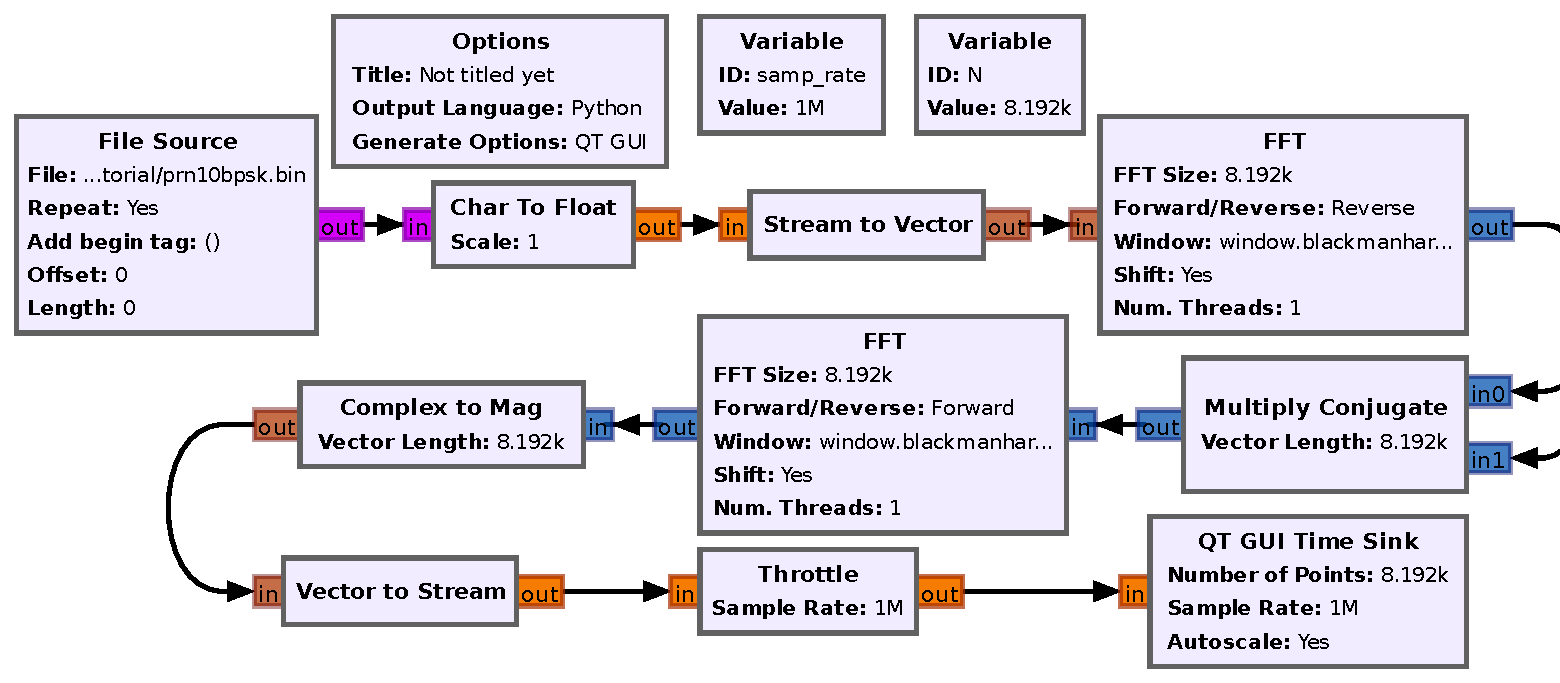
\includegraphics[width=\linewidth]{amaranth_PRNcorrelation.pdf}

Flowchart
\end{minipage}
\begin{minipage}{.49\linewidth}
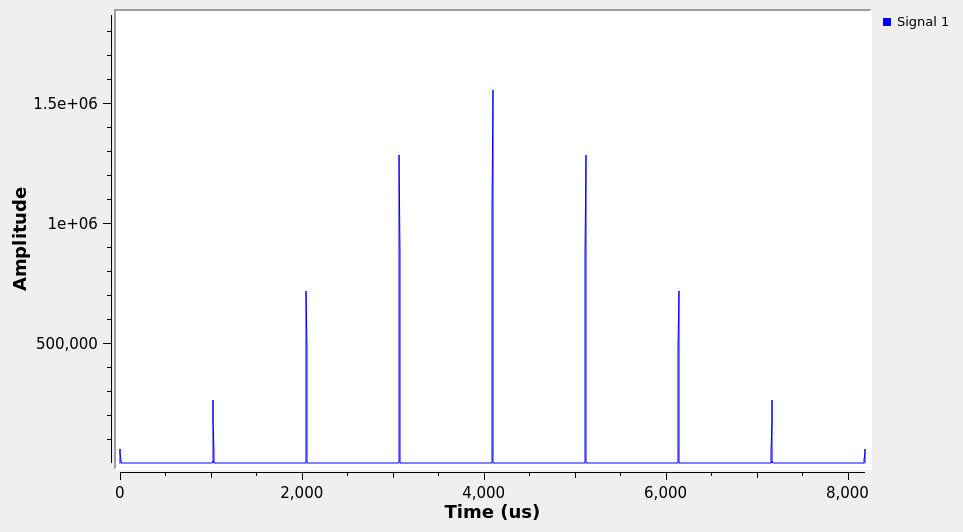
\includegraphics[width=\linewidth]{amaranth_PRNcorrelation_output.png}

~\hfill Result (correlation peak every 1023~sample delays)~~~~~
\end{minipage}
\end{minipage}

\vspace{0.2cm}
File Source reads the file generated by Amaranth (1~byte/PRN chip -- use Packed
to Unpacked if 1~bit/PRN chip)
\end{frame}

\begin{frame}[fragile,noframenumbering]\frametitle{Transposition to radiofrequency band: BPSK}

\parbox{1.05\linewidth}{
\begin{itemize}
\item Generating the Numerically Controlled Oscillator (NCO) as LO, selecting the clock source
\vspace{-0.1cm}
\item Mixing the baseband signal to LO to generate the RF signal: BPSK, $\varphi=\{0,\pi\}\Rightarrow
s=\{-1,1\}\in\mathbb{R}$
\item Receiving and characterizing the RF signal (auto-correlation of the signal collected by the B210)
\begin{itemize}
\item $N$-th power of N-PSK recovers the carrier
\item Costas Loop to cancel FPGA clock to B210 clock offset
\item Displaying the constellation, $p$ samples/symbol including transitions
\item Symbol Synchronization block and displaying the constellation, 1 sample/symbol
\end{itemize}
\end{itemize}
}

\vspace{-0.15cm}
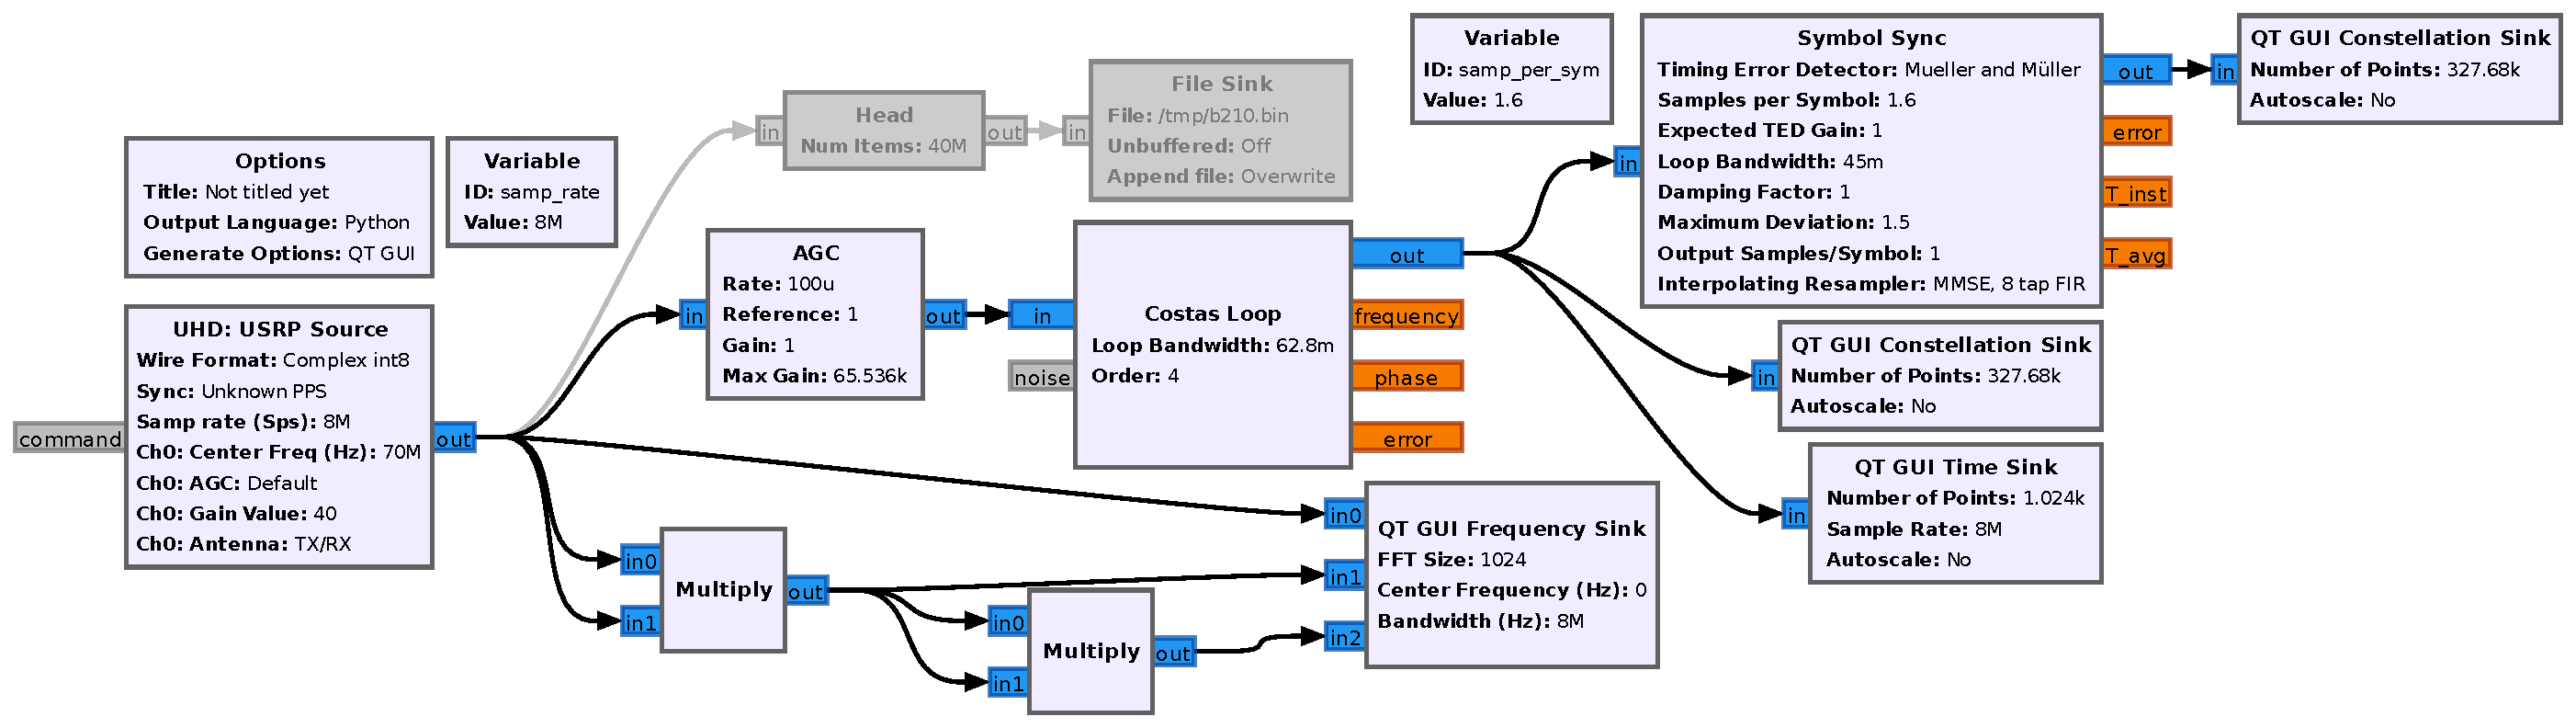
\includegraphics[width=\linewidth]{b210.pdf} % b210_constellation}

\vspace{-0.15cm}
Correlation with the local copy of the code: interpolate the code sequence to match the sampling rate:
\verb~code=repelems(code,[[1:length(code)] ; ones(1,length(code))*2]);~
\end{frame}

\begin{frame}[fragile,noframenumbering]\frametitle{Transposition to radiofrequency band: QPSK}

\begin{minipage}[t]{\linewidth}
\begin{minipage}{.39\linewidth}
\begin{itemize}
\item BPSK only uses half the bandwidth by modulating I and keeping Q null
\item Double digital bandwidth at the same analog bandwidth: QPSK 
\item $\varphi=\{0,\pi/2,\pi,3\pi/2\}\Rightarrow s=\{j,-1,-j,1\}$ requires full complex modulator ...
\item ... and LO$< f_{FPGA}/4$
\item Practical implementation using Amaranth
\item Receiving and characterizing the RF signal (auto-correlation of the signal collected by the B210)
\end{itemize}
\end{minipage}
\begin{minipage}{.59\linewidth}
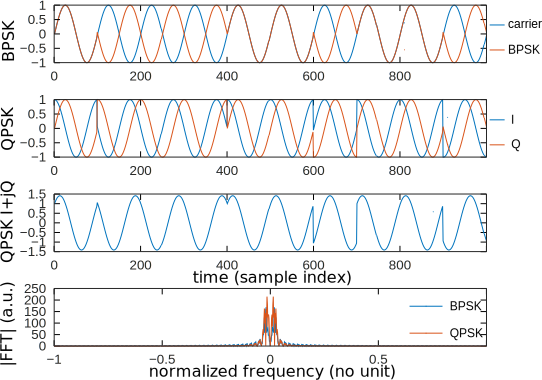
\includegraphics[width=1.13\linewidth]{bpsk_qpsk}
\end{minipage}
\end{minipage}
\end{frame}

\begin{frame}[fragile,noframenumbering]\frametitle{Transposition to radiofrequency band: Frequency Modulation (FM)}

\begin{itemize}
\item FM modulation: incoherent (no need to recover the carrier) modulation 
scheme still popular with ham radio (NBFM) and commercial broadcast (WBFM)
\item $s(t)=\cos(2\pi f_c t+f_\Delta \int x(t)dt)$ with $f_\Delta$ the
frequency deviation induced by signal $x$ to be transmitted
\item if $x(t)=\cos(2\pi f_m t)$ (one spectral component of signal $x$) then
$s(t)=\cos(2\pi f_c t+\frac{f_\Delta}{f_m}\sin(2\pi f_mt))$ 
\item $\Rightarrow$ tune $f_c$ with $\sin(2\pi f_mt)$ to transmit the 
FM-modulated tone $f_m$
\item $f_\Delta/f_m\ll 1$: NBFM, $f_\Delta/f_m\gg 1$: WBFM
\item Practical implementation using Amaranth: generate a sine wave at $f_m$
and update the LO frequency with this signal
\end{itemize}
\end{frame}

\begin{frame}[fragile,noframenumbering]\frametitle{Conclusion}

PEUT-ON CONCLURE EN SYNTHETISANT LE MEME PROJET SUR UNE AUTRE BOARD ?

Supporting resources available at
{\url{https://github.com/oscimp/amaranth_twstft}}
\end{frame}

\end{document}
